\section{Uma Linguagem} %------------------------------------------------------
\label{sec:aprendendo}

\begin{margintable}\vspace{.8in}\footnotesize
  \caption{Sumário da \textsc{Part II}}
  \medskip
  \begin{tabularx}{\marginparwidth}{|X}
    \textbf{\sffamily \textcolor{azulUFRB}{Seção}~\ref{sec:aprendendo}}.    {\sffamily Uma Linguagem} \\
  \end{tabularx}
\end{margintable}

A aquisição de uma linguagem não é algo imediato, para a maioria das pessoas; e,
o \LaTeX{} é uma linguagem (de marcação).
Isso implica que há uma \textsf{estrutura} e \textsf{simbologia} características.

Vimos na Subseção~\ref{subsec:latex-word} que o \hologo{LaTeX} é uma linguagem 
que envolve \textit{códigos} e \textit{texto}.
Sua estruturação é diferente de sistemas \textsf{WYSYWYG} (como o Word) e, à
primeira vista, demanda um "esforço técnico"\, maior no início do aprendizado, 
mesmo para documentos simples.
Mas, à medida que a complexidade do documento aumenta, o esforço empregado ao 
usar o \LaTeX{} é menor, quando comparado à sistemas \textsf{WYSYWYG}, para 
produzir o esse mesmo documento.
A Figura~\ref{fig:latex-vs-word} mostra um vislumbre dessa ideia, embora seja
apenas hipotética.

\begin{figure}[!htbp]
  \centering
  \caption{Complexidade do Documento vs Esforço empregado}
  \label{fig:latex-vs-word}
  \medskip
  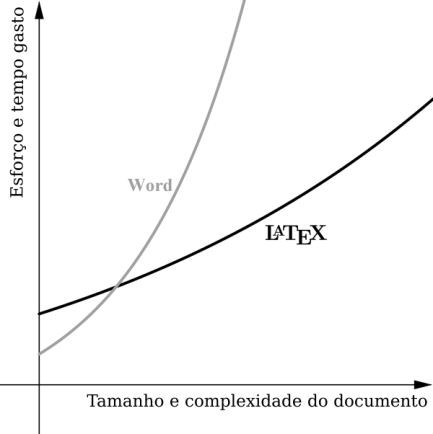
\includegraphics[width = 0.6\linewidth]{figs/latex-vs-word.png}
  
  {\small \textbf{Fonte:} \url{https://latexcfp.wordpress.com/}}
\end{figure}

\begin{marginfigure}
  
\includegraphics[width = \linewidth]{piada-latex.png}
  
  {
    \sffamily
    \textit{Seu artigo não faz nehum sentido para 
    mim, mas é a coisa mais linda que eu já vi!}
    (Tradução livre e suavizada \emoji{grinning-face-with-sweat})
  }
  
  {\textsf{\textbf{Fonte:}} \href{http://nvisnjic.com/2015/01/13/mathjax-magic.html}{The magic of LaTeX.}}
\end{marginfigure}

Além disso, é notável a beleza da composição tipográfica final, em especial -- mas
não necessariamente, quando o documento envolve equações matemáticas.

\subsection{Um pouco sobre a estruturação do LaTeX} %--------------------------

Antes de aprendermos os símbolos perinentes dessa linguagem, é interessante 
conhecermos um pouco de sua estruturação.

Um comando no \LaTeX{} sempre começa com uma barra invertida: \textbackslash.
Tal comando pode está inserido em \textsf{modo texto} ou em \textsf{modo matemático}.
\sidenote{
  Existe toda uma sintaxe para o \textsf{modo matemático}, que vamos deixar para
  abordar em outra seção.
}
Por exemplo, quando escrevemos \verb|\LaTeX|, com o "L", "T"\, e "X"\, maiúsculos, 
o resultado depois da compilação é: \LaTeX.
Mas, se digitarmos \verb|\Latex| uma mensagem de erro será mostrada, visto que 
esse comando não vem por padrão definido.

Tal exemplo já nos mostra uma outra característica da estruturação da linguagem 
que estamos conhecendo: ela é \textit{case sensitive}, ou seja, é sensível à
letras maiúsculas e menúsculas.
O comando \verb|\LaTeX| é difernete do comando \verb|\latex|, que é difernte do
comando \verb|\Latex|.
\sidenote{
  \small \texttt{\textbackslash LaTeX} $\neq$ \texttt{\textbackslash Latex} $\neq$ \texttt{\textbackslash latex}
}

\begin{atencao}{Atenção!}{\exclamacao}
  Inclusive, essa é uma das grandes fontes de erro de quem está começando no 
  \LaTeX: a digitação de um comando de forma errada é muito comum!
\end{atencao}

Quando escrevemos um texto, precisamos saber qual tipo de texto ele representa.
Poderia ser um artigo; um livro; uma nota de aula; um relatório; um protocolo;
uma revista; uma apresentação; etc.
Cada uma dessas \textsf{classes} possui características instrínsecas: um artigo 
não possui capítulos, mas seções; o que é diferente de um livro, que possui 
essas duas estruturas.



